\section{Master dissertation review}

\begin{frame}
\frametitle{System modelling with Simulink}
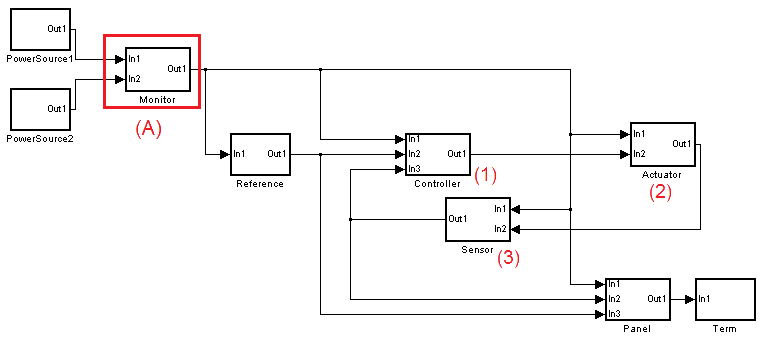
\includegraphics[width=\linewidth]{acsBlockDiagrams}
\end{frame}

\begin{frame}
\frametitle{Fault Tolerance, Failure Logic, Safety Analysis}
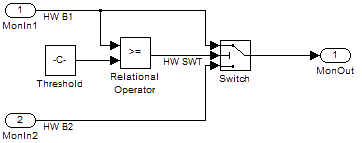
\includegraphics[height=0.4\textheight]{blockDiagramMonitorInternals}\par
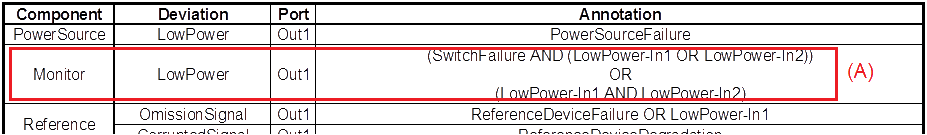
\includegraphics[width=\linewidth]{acsAnnotations}
\end{frame}

\begin{frame}[fragile]
\frametitle{\CSPM to inject faults and obtain fault traces}
From:\\
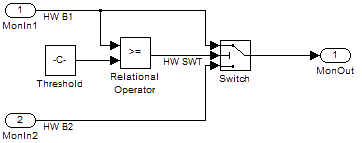
\includegraphics[height=0.3\textheight]{blockDiagramMonitorInternals}\par

We obtain traces with faults:
{\tiny
\begin{itemize}
  \item \verb|failure.Hardware.N04_RelationalOperator| -- HW SWT \onslide<2->{(S)}
  \item \verb|failure.Hardware.N04_MonIn1| -- HW B1 \onslide<2->{(A)}
  \item \verb|failure.Hardware.N04_MonIn2| -- HW B2 \onslide<2->{(B)}
\end{itemize}
}

\end{frame}

\begin{frame}[fragile]
\frametitle{Faults trace example}
Two of the 64 traces are:
\begin{snippetcspm}[0]
TRACE 1:
failure.Hardware.N04_MonIn2.1.EXP.I.5
failure.Hardware.N04_MonIn2.1.ACT.OMISSION
failure.Hardware.N04_RelationalOperator.1.EXP.B.true
failure.Hardware.N04_RelationalOperator.1.ACT.B.false
out.1.OMISSION

TRACE 2:
failure.Hardware.N04_MonIn1.1.EXP.I.5
failure.Hardware.N04_MonIn1.1.ACT.OMISSION
failure.Hardware.N04_MonIn2.1.EXP.I.5
failure.Hardware.N04_MonIn2.1.ACT.OMISSION
out.1.OMISSION
\end{snippetcspm}
\footnotesize
\begin{itemize}
  \item Combine each trace with conjunctions: $B \land S$, $A \land B$, \ldots
  \item Combine all traces with disjunctions: $(B \land S) \lor (A \land B) \lor \ldots$
  \item The complete failure logic after simplification is exactly the supplied by Embraer: \alert<4>{$(A \land B) \lor (S \land (A \lor B))$}
  \item <2-> Note that we ignore events order in each trace, because Boolean AND is commutative.
  \item<3-> Some traces appear in a specific order: $A$ then $S$, but not $S$ then $A$.
\end{itemize}

\onslide<4>{\tikzoverlay[text width=3cm] at (3.8cm,2.7cm) {a.k.a structure function or structure expression};}
\end{frame}